%% -*- coding: utf-8 -*-
\documentclass[12pt,a4paper]{report}
\usepackage[left=2cm,right=2cm,
    top=2cm,bottom=2cm,bindingoffset=0cm]{geometry} 
\usepackage[utf8]{inputenc}
\usepackage[english,russian]{babel}
\usepackage{indentfirst}
\usepackage{misccorr}
\usepackage{graphicx}
\usepackage{amsmath}
\usepackage{amsfonts}
\usepackage{amssymb}
\setcounter{page}{2}
\begin{document}

\begin{titlepage}
\newpage
  \begin{center}
     
    Санкт-Петербургский Политехнический Университет Петра Великого \\
    
    Институт компьютерных наук и технологий \\
    
    Кафедра компьютерных систем и программных технологий
    \end{center}
    
    \vspace{15em}
    \begin{center}
    \textsc{Лабораторная работа №8}\\
    \vspace{5mm}
    \textsc{Модель телекоммуникационного канала}
    	
   \end{center}
\vspace{10em}

\newlength{\ML}
\settowidth{\ML}{«\underline{\hspace{0.7cm}}» \underline{\hspace{2cm}}}
\hfill\begin{minipage}{0.45\textwidth}
\vfill
  Руководитель \\
  \\
  \underline{\hspace{\ML}} Богач Н.\,В.\\
 
\end{minipage}%
\bigskip

\hfill\begin{minipage}{0.45\textwidth}
  Выполнил\\
  \\
  \underline{\hspace{\ML}} Солдатова Е.\,И.\\
  группа 33501/3
\end{minipage}%

\vspace{\fill}
\begin{center}
    
  Санкт-Петербург\\
   2018 
\end{center}
\end{titlepage}

\paragraph{1. Цель работы\\\\}
Разработка модели телекоммуникационного канала.

\paragraph{2. Постановка задачи\\\\}
По имеющейся записи сигнала из эфира и коду модели передатчика создать модель приемника, в которой найти позицию начала
пакета и, выполнив операции демодуляции, деперемежения и декодиро-
вания, получить передаваемые параметры: ID, период, и номер пакета.
Известно, что ID = 4, период 100 мс, номер пакета 373. Запись сделана с передискретизацией 2, т.е. одному BPSK символу соответствуют 2 лежащих друг за другом отсчета в файле. Запись сделана на нулевой частоте и представляет из себя последовательность 32-х битных комплексных отсчетов, где младшие 16 бит вещественная часть, старшие 16 бит – мнимая часть.

\paragraph{3. Теоретическая часть \\\\}
Описание работы канала:
Пакетный сигнал длительностью 200 мкс состоит из 64 бит полезной ин-
формации и 8 нулевых tail-бит. В нулевом 16-битном слове пакета пере-
дается ID, в первом - период излучения в мс, во втором – сквозной номер пакета, в третьем - контрольная сумма (CRC-16). На передающей стороне пакет сформированный таким образом проходит следующие этапы
обработки:
\begin{enumerate}
\item Помехоустойчивое кодирование сверточным кодом с образующими
полиномами 753, 561( octal ) и кодовым ограничением 9. На выходе
кодера количество бит становится равным 144.
\item Перемежение бит. Количество бит на этом этапе остается неизмен-
ным.
\item Модуляция символов. На этом этапе пакет из 144 полученных с
выхода перемежителя бит разбивается на 24 символа из 6 бит. Ге-
нерируется таблица функций Уолша длиной 64 бита. Каждый 6-
битный символ заменяется последовательностью Уолша, номер которой равен значению данных 6-ти бит. Т.о. на выходе модулятора
получается 24 * 64 = 1536 знаковых символов.
\item Прямое расширение спектра. Полученная последовательность из
1536 символов периодически умножается с учетом знака на ПСП
длиной 511 символов. Далее к началу сформированного символьного пакета прикрепляется немодулированная ПСП. Т.о. символьная
длина становится равной 1747. Далее полученные символы модулируются методом BPSK .
\end{enumerate}
\newpage
\paragraph{4. Ход работы \\\\}
Текст программы:\\

\begin{figure}[h!]
\center{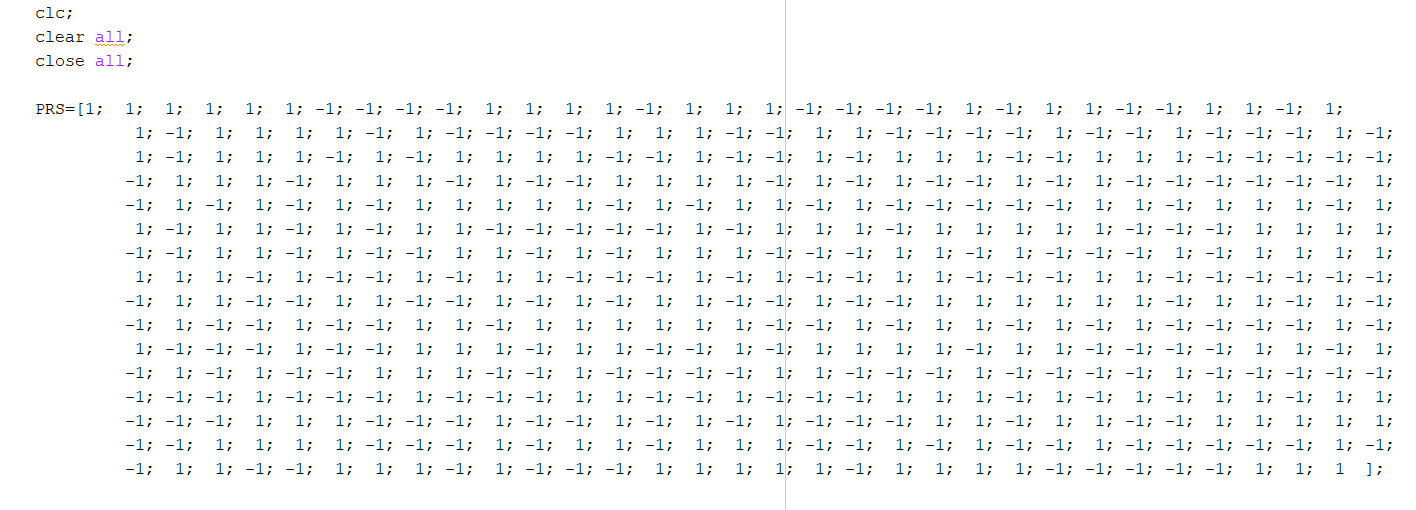
\includegraphics[width=1\linewidth]{1}}
\end{figure}
\begin{figure}[h!]
\center{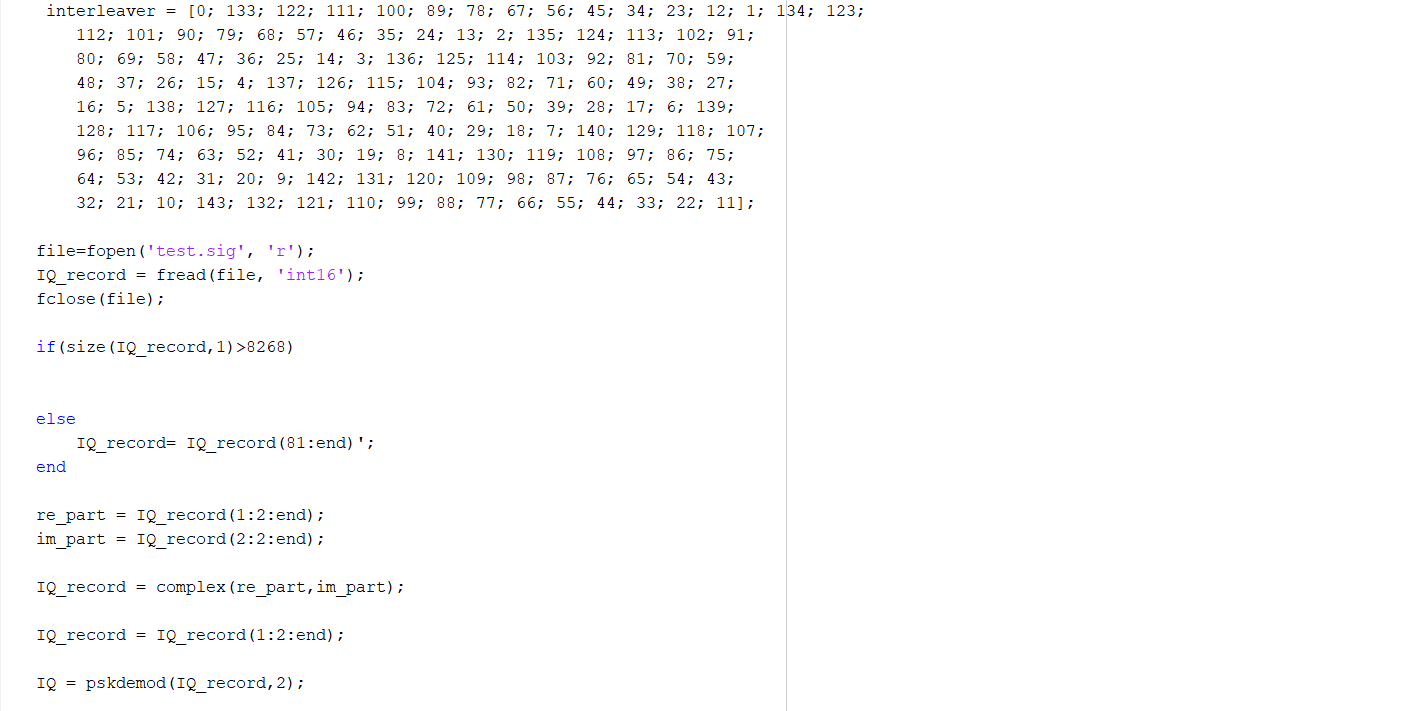
\includegraphics[width=1\linewidth]{2}}
\end{figure}
\begin{figure}[h!]
\center{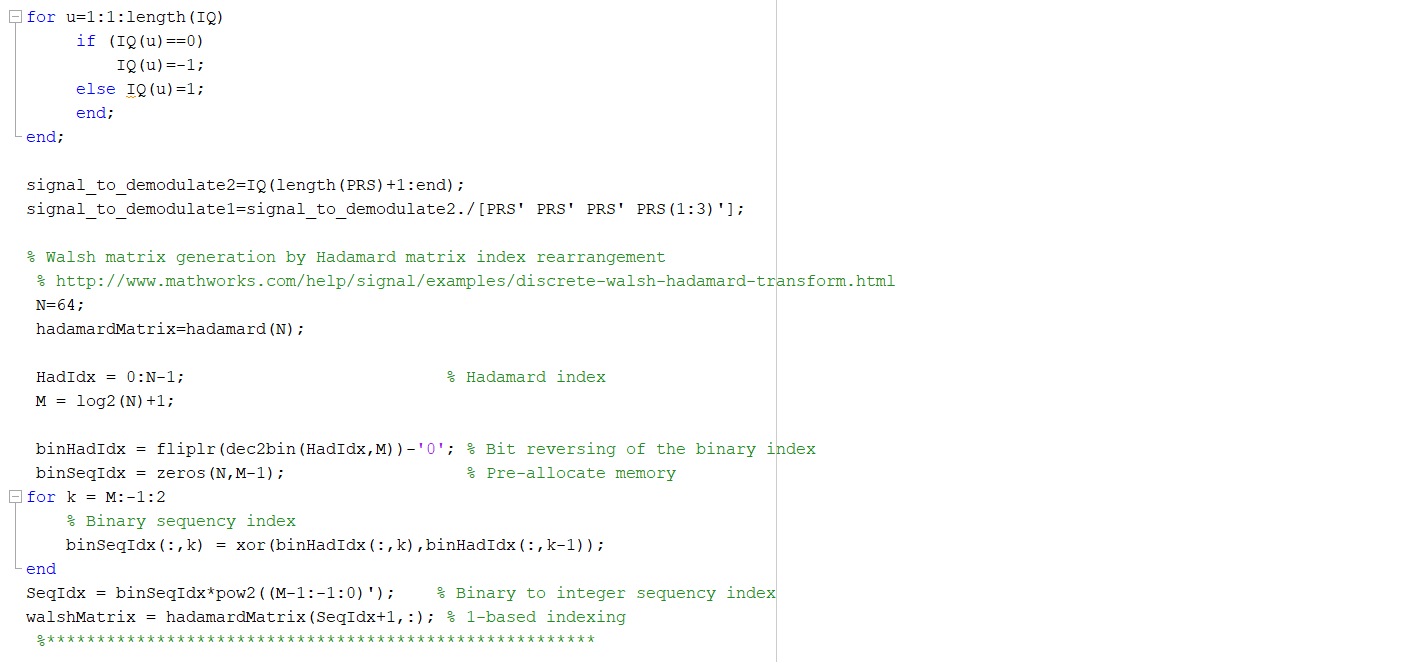
\includegraphics[width=1\linewidth]{3}}
\end{figure}
\begin{figure}[h!]
\center{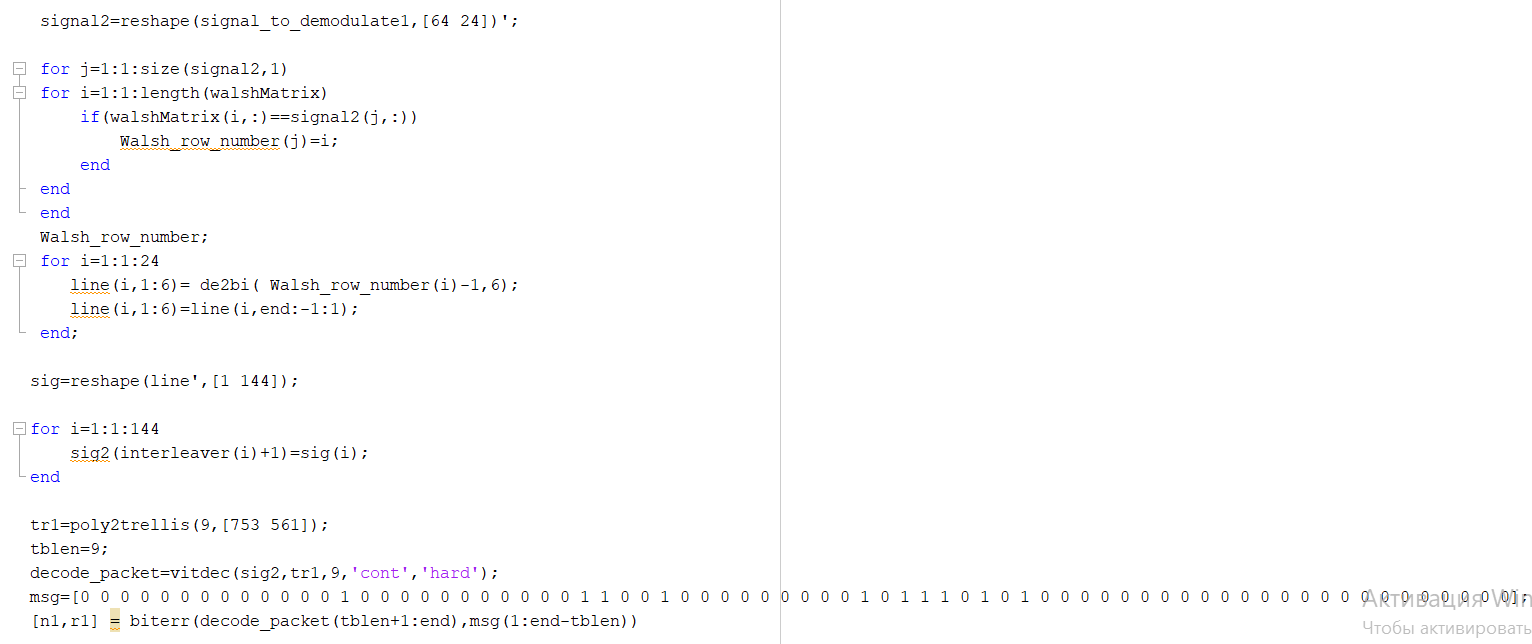
\includegraphics[width=1\linewidth]{4}}
\end{figure}
\newpage
\paragraph{5. Выводы \\\\}
В ходе данной работы было разработано, промоделировано, отлажено и настроено устройство приема данных согласно конкретному техническому заданию. 

Модель приемника была создана на основе модели передатчика: были проведены обратные действия. Когда на передатчике были проведены операции модуляции, перемежения и кодирования параметров, на приемнике были выполнены демодуляциия, деперемежение и декодирование, были получены передаваемые параметры.

\end{document}